

\section{引言}
计算机与网络技术的高速发展,特别是面向对象技术的出现,使得C++的软件开发得到了迅速普及。

本课题主要………………




\section{线性表的基本理论知识}
\subsection{线性表的定义}
线性表是最简单、最常用\cite{Rouse1974Monitoring}的一种数据结构。线性表\cite{贾永红2010数字图像处理}是n(n>=0)个数据元素的有限序列。

……。
\subsection{线性顺序表}
线性表的顺序存储结构的特点是为表中相邻的元素$a_i$和$a_{i+1}$ 赋以相邻的存储位置。
\subsubsection{三级标题名}
\subsubsection{三级标题名}
\begin{itemize}
        \item [(1)] 三级以下标题
\end{itemize}




\subsection{线性链表}

线性表的链式存储结构的特点是用一组任意的存储单元存储线性表的数据元素(这组元素可以是连续的,也可以是不连续的)。


\begin{definition}
线性表的定义为
\end{definition}


\begin{theorem}
设sxibaxabxugbuaxbsusabx
\begin{proof}
由线性表的特殊定义可得。
\end{proof}
\end{theorem}
设sxibaxabxugbuaxbsusabx
\begin{lemma}
设sxibaxabxugbuaxbsusabx
\begin{proof}
由线性表的特殊定义可得。
\end{proof}
\end{lemma}



\section{设计的主体内容}
在着手进行上机设计之前首先做好大量准备:应熟悉课题,进行调查研究,收集国内、外资料、分析研究;交互界面的设计和实现。

……。
\subsection{系统结构的设计}
……。
\subsection{交互界面的设计和实现}
交互界面的设计应遵循………。
\begin{equation}
        b\approx\frac{L_0}{\rho\tan(\theta_0)+z_0}
\end{equation}
式中,$z_0$为\textit{Goos-Hanchen}位移;$\theta_0$为光波的入射角。

由公式(3-1)可以看出………。
\subsection{线性表的OOP序设计}
计算机内部可以采用两种不同方法来表示一个线性表,它们分别是顺序表示法和链表表示法。

……。

过阻尼响应如图\ref{guozuni}所示。
\begin{figure}[htbp]
\centering

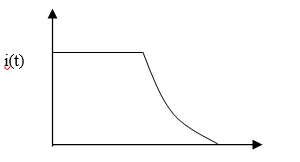
\includegraphics{./figure/guozuni.png}
\caption{过阻尼响应}
\label{guozuni}
\end{figure}
\subsubsection{线性表的顺序存储的实现}
……

以上是顺序表的实现过程,第1-16行包含了list类的说明,接下来是成员函数的定义。

……。
\subsubsection{线性表的链表存储的实现}
……

链表的实现包括两个类定义,第一个是link类,第二个是list类。由于一个链表由若干个单独的链结点对象组成,因此一个链结点应当作为单独的link类实现。

……

……

\section{实验及结果分析}
例如由于起初未能真正掌握各种控件的功能,我设想是要一个下拉菜单,但是学识肤浅的我试了很多种就是达不到我要的效果,……。

……

关于……的影响如表\ref{data_table}所示。

……

\begin{table}[htbp]
        \small
        \newcommand{\tabincell}[2]{\begin{tabular}{@{}#1@{}}#2\end{tabular}}
        \centering
        \caption{激光入射功率密度对导轨滚道表面硬化层深和显微硬度的影响}
        \begin{tabular}{ccccc}
                \toprule
                试验编号 & 功率密度 & 辐照时间 & 显微硬度       & 硬化层深\\ \midrule
                t-1	&6.37×103	&0.067	&570,456	&0.354\\
                t-2	&6.37×103	&0.067	&570,456	&0.354\\
                t-3	&6.37×103	&0.067	&570,456	&0.354\\
                t-4	&6.37×103	&0.067	&570,456	&0.354\\
                t-5	&6.37×103	&0.067	&570,456	&0.354\\ \bottomrule
        \end{tabular}
        \label{data_table}
\end{table}


鉴于表格复杂性,此处提供了可换行示例表见表\ref{kehuanhang}
\begin{table}[htbp]
        \small
        \newcommand{\tabincell}[2]{\begin{tabular}{@{}#1@{}}#2\end{tabular}}
        \centering
        \caption{可换行示例表}
        \begin{tabular}{ccc}
                \toprule
                1	& 2& 3\\ \midrule
                1&\tabincell{c}{3}&6\\
                1&\tabincell{c}{3}&6\\
                \tabincell{c}{2}&\tabincell{c}{4444444444\\5555555555}&\tabincell{c}{6}
                \\ \bottomrule
        \end{tabular}
        \label{kehuanhang}
        \vspace{0.5em}
\end{table}

此处也提供了多列合并示例表如表\ref{duoliehebing}
\begin{table}[htbp]
        \small
        \centering
        \caption{多列合并示例表}
        \begin{tabular}{ccccccccc}
                \toprule
                & \multicolumn{2}{c}{ZZ}& \multicolumn{6}{c}{XX}\\
                \cmidrule(lr){2-3} \cmidrule(lr){4-9}
                &   &   & \multicolumn{2}{c}{CC}&\multicolumn{4}{c}{VV}\\
                \cmidrule(lr){4-5} \cmidrule(lr){6-9}
                &   &   &   &   & \multicolumn{3}{c}{BB}&NN\\
                \cmidrule(lr){6-8} \cmidrule(lr){9-9}
                & A &S	&D &F &G &H &J &K \\ \midrule
                Q&$\surd$&$\surd$&   &   &   &    & &\\
                T&	&		& $\surd$ & $\surd$   &   &  &$\surd$     &\\
                Y&	&		& $\surd$ & $\surd$   &   &  &    &$\surd$ \\ \bottomrule
        \end{tabular}
        \label{duoliehebing}
\end{table}

\section{结论}
        本课题采用C++语言、面向对象的设计方法实现数据结构的重要算法。

        …….

        而且还存在着许多不足之处。如:
